\documentclass[10pt]{article}

\usepackage[english]{babel}
\usepackage[utf8x]{inputenc}
\usepackage[fleqn]{amsmath}
\usepackage{amssymb}
\usepackage{amsfonts}
\usepackage{graphicx}
\usepackage[ruled,linesnumbered,noend]{algorithm2e}
\usepackage{empheq}
\usepackage{float}
\usepackage{enumitem}
\usepackage{tikz}
\usepackage[colorlinks=true,urlcolor=blue]{hyperref}

\title{Introduction to Machine Learning, Fall 2014 - Exercise session III}
\author{Rodion ``rodde'' Efremov \\ 013593012}

\begin{document}
 \maketitle

\color{blue}
\section*{Problem 1 (3 points)}
Consider a binary classification task with two classes, `+' and `-'. The desired prediction is either one of the two classes, or alternatively answering `don't know', with the following cost matrix:
\begin{center}
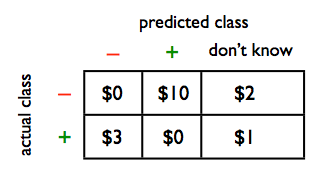
\includegraphics{cost_table}
\end{center}
The goal is to minimize the expected cost (which is also the long-term average cost). You are given a classification method that returns a probabilistic prediction, i.e. for each new object the existing method gives you the probability $\alpha$ that the object belongs to class `+' (and hence $1 - \alpha$ is the probability that the object belongs to class `-').
 
Give the optimal policy for answering `+', `-', or `don't know' for each object, as a function of the value of $\alpha$. That is, for any given value of $\alpha$ (for $0 \leq \alpha \leq 1$) what is the best answer of the three possibilities?

\color{blue}
\section*{Problem 2 (3 points)}
In a binary classification task we are trying to classify the objects \textbf{x} into classes $y = 1$ and $y = 0$. We are here using probabilistic predictions, so for each new object we are required to output our probability $b = P(y = 1 | \textbf{x})$, with $0 \leq b \leq 1$. We are using the following quadratic cost function:
\begin{align}
C(y, b) = 
\begin{cases}
(b - 1)^2,  & \mbox{if } y = 1\\
b^2,          & \mbox{if } y = 0
\end{cases}
\end{align}
Obviously, if the value of $y$ is 1, the lowest cost (0) is obtained when $b = 1$. Similarly, if the value of $y$ is 0, the lowest cost (0) is obtained when $b = 0$, so the cost function seems to encourage appropriate behaviour. In fact, the cost function is \textit{proper}. Show this. (Hint: Assume that the true probability that $y = 1$ is $a$ (so the true probability that $y = 0$ is $1 - a$), and show that the expected cost is minimized for $b = a$.)

\color{black}
\noindent So we suppose that $P(y = 1 | \textbf{x}) = b$ and $P(y = 0 | \textbf{x}) = 1 - b$. Let the actual probabilities be $P(y = 1 | \textbf{x}) = a$ and $P(y = 0 | \textbf{x}) = 1 - a$. Now the expected cost is
\begin{align*}
E\{C\} &= aC(1, b) + (1 - a)C(0, b) \\
           &= a(b - 1)^2 + (1 - a)b^2 \\
           &= a(b^2 - 2b + 1) + b^2 - ab^2 \\
           &= ab^2 - 2ab + a + b^2 - ab^2 \\
           &= b^2 - 2ab + a.
\end{align*}
To minimize $E\{C\}$, we take the first derivative with respect to $b$, that is
\[
2b - 2a = 2(b - a).
\]
The second derivative with respect to $b$ is 2, which implies that at point $b = a$ $E\{C\}$ is minimized, and so the cost function is indeed proper.

\color{blue}
\section*{Problem 3 (3 points)}
The figure below shows the class conditional probability densities $p(\textbf{x} | y)$ of 3 different classes ($y = 0$, $y = 1$, and $y = 2$): Each of the class conditionals is a uniform density over the corresponding rectangle. (For example, all vectors $\textbf{x}$ belonging to class $y = 0$ have attribute values $x_1 \in [1, 4]$ and $x_2 \in [3, 5]$, and these vectors are uniformly distributed within this rectangle.) Additionally we know that the marginal probabilities of the classes are $P(y = 0) = 0.2$, $P(y = 1) = 0.7$, $P(y = 2) = 0.1$. For each of the indicated points $\textbf{x}_1, \dots, \textbf{x}_5$, compute the posterior probability distribution over the three classes. (That is, when observing a new vector $\textbf{x}_i$, what is the probability that it belongs to class $y = 0$, to class $y = 1$, or to class $y = 2$? Remember that these probabilities should sum to one.)

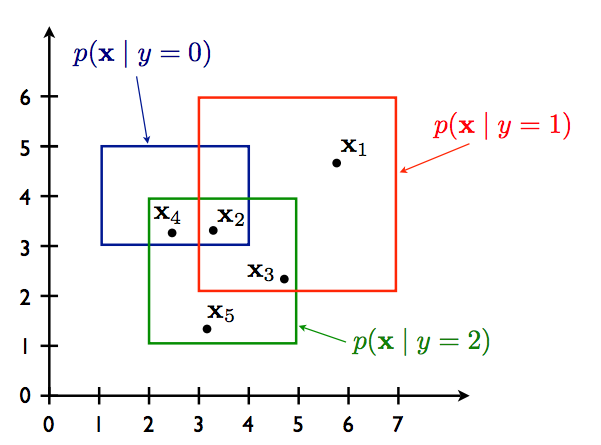
\includegraphics[width=\textwidth,keepaspectratio]{rectangles}

\color{black}
\noindent It follows immediately from the figure that points $\textbf{x}_1$ and $\textbf{x}_5$ will be ``classified'' with probability 1 to classes $y = 1$ and $y = 2$, respectively. Before considering the other 3 points, we state what we know or can calculate. The marginal probabilities are as follows
\begin{align*}
P(y = 0) &= 0.2, \\
P(y = 1) &= 0.7, \\
P(y = 2) &= 0.1.
\end{align*}
The total area covered in the figure is 24 units of area, so we can easily compute the following probabilities:
\begin{align*}
&P(\textbf{x} \, | \, y = 0) = 6 / 24 = 0.25, \\
&P(\textbf{x} \, | \, y = 1) = 16 / 24 = 0.\bar{6}, \\
&P(\textbf{x} \, | \, y = 2) = 9 / 24 = 0.375. 
\end{align*}

\subsection*{Point $\textbf{x}_3$}
The probabilities we are interested in are
\begin{itemize}
  \item $P(y = 0 \, | \, \textbf{x}_3) = 0$ as the point is outside the class $y = 0$,
  \item $P(y = 1 \, | \, \textbf{x}_3)$,
  \item $P(y = 2 \, | \, \textbf{x}_3)$.
\end{itemize}
The total probability is
\begin{align*}
P(\textbf{x}) &= \sum_{i = 0}^2 P(\textbf{x} \, | \, y = i)P(y = i) \\
                    &= \overbrace{P(\textbf{x} \, | \, y = 0)}^0 P(y = 0) + P(\textbf{x} \, | \, y = 1)P(y = 1) + P(\textbf{x} \, | \, y = 2)P(y = 2) \\
                    &= 0.\bar{66} \times 0.7 + 0.375 \times 0.1 \\
                    &\approx 0.50417.
\end{align*}
\begin{align*}
P(y = 1 \, | \, \textbf{x}_3) &= \frac{ P( \textbf{x}_3 \, | \, y = 1)P(y = 1)}{ P(\textbf{x}) } \\
                                          &= \frac{ 0.\bar{66} \times 0.7}{0.50417} \\
                                          &\approx 0.92562. \\
P(y = 2 \, | \, \textbf{x}_3) &= \frac{P(\textbf{x}_3 \, | \, y = 2)P(y = 2)}{P(\textbf{x})} \\
                                          &= \frac{0.375 \times 0.1}{0.50417} \\
                                          &\approx 0.074380. 
\end{align*}
Note that two above probabilities sum to 1, as expected.
\subsection*{Point $\textbf{x}_4$}
The probabilities we are interested in here are
\begin{itemize}
  \item $P(y = 0 \, | \, \textbf{x}_4)$,
  \item $P(y = 1 \, | \, \textbf{x}_4) = 0$ as the point is outside the class $y = 1$,
  \item $P(y = 2 \, | \, \textbf{x}_4)$.
\end{itemize}
The total probability is
\begin{align*}
P(\textbf{x}) &= \sum_{i = 0}^2 P(\textbf{x} \, | \, y = i)P(y = i) \\
                    &= P(\textbf{x} \, | \, y = 0) P(y = 0) + \overbrace{P(\textbf{x} \, | \, y = 1)}^0 P(y = 1) + P(\textbf{x} \, | \, y = 2)P(y = 2) \\
                    &= 0.25 \times 0.2 + 0.375 \times 0.1 \\
                    &\approx 0.0875.
\end{align*}
\begin{align*}
P(y = 0 \, | \, \textbf{x}_4) &= \frac{ P( \textbf{x}_4 \, | \, y = 0)P(y = 0)}{ P(\textbf{x}) } \\
                                          &= \frac{ 0.25 \times 0.2}{0.0875} \\
                                          &\approx 0.57143 \\
P(y = 2 \, | \, \textbf{x}_4) &= \frac{P(\textbf{x}_4 \, | \, y = 2)P(y = 2)}{ P(\textbf{x}) } \\
                                          &= \frac{0.375 \times 0.1}{0.0875} \\
                                          &\approx 0.42857. 
\end{align*}
\subsection*{Point $\textbf{x}_2$}
The probabilities we are interested in are
\begin{itemize}
 \item $P(y = 0 \, | \, \textbf{x}_2)$,
 \item $P(y = 1 \, | \, \textbf{x}_2)$,
 \item $P(y = 2 \, | \, \textbf{x}_2)$,
\end{itemize}
Also,
\begin{align*}
P(\textbf{x}) &= \sum_{i = 0}^2 P(\textbf{x} \, | \, y = i) P(y = i) \\
                    &= 0.2 \times P(\textbf{x} \, | \,  y = 0) + 0.7 \times P(\textbf{x} \, | \, y = 1) + 0.1 \times P(\textbf{x} \, | \, y = 2) \\
                    &= 0.2 \times 0.25 + 0.7 \times 0.\bar{6} + 0.1 \times 0.375 \\
                    &\approx 0.55417.
\end{align*}

\begin{align*}
   P(y = 0 \, | \, \textbf{x}_1) &= \frac{P(\textbf{x} \, | \, y = 0)P(y = 0)}{P(\textbf{x})} \\
                                             &= \frac{0.25 \times 0.2}{0.55417} \\
                                             &= 0.090255. \\
   P(y = 1 \, | \, \textbf{x}_1) &= \frac{P(\textbf{x} \, | \, y = 1)P(y = 1)}{P(\textbf{x})} \\
                                             &= \frac{0.\bar{6} \times 0.7}{0.55417} \\
                                             &= 0.8421. \\
   P(y = 2 \, | \, \textbf{x}_1) &= \frac{P(\textbf{x} \, | \, y = 2)P(y = 2)}{P(\textbf{x})} \\
                                             &= \frac{0.375 \times 0.1}{0.55417} \\
                                             &= 0.067669. 
\end{align*}
Once again, the above probabilities sum to one, so they define a valid probability distribution.

\color{blue}
\section*{Problem 4 (15 points)}
In this exercise we implement an extremely simple prototype-based classifier to classify handwritten digits from the MNIST dataset, and compare that to a nearest-neighbor classifier.

\color{black}
The included \texttt{ex3.m} file contains well documented version of the code following. Also, if the \texttt{cd} command in the file is corrected to your path to MNIST data, it can be run with the \texttt{run('ex3.m')} command.

\color{blue}

\begin{itemize}
\item[(a)] Download the MNIST data from the course web page. In addition to the actual data, the package contains some functions for easily loading the data into Matlab/Octave/R and for displaying digits. See the README files for details. Load the first $N=5,000$ images using the provided function.

\color{black}
First we need to get to the directory containing the \texttt{loadmnist.m} file, run it, and load 5000 images along their class labels.
\begin{verbatim}
cd /path/to/mnist
run('loadmnist.m');
[X y] = loadmnist(5000);
\end{verbatim}
Now the matrix $X$ contains an image at each row (\texttt{X(i,:)} is the $i$th image).

\color{blue}
\item[(b)] Use the provided functions to plot a random sample of 100 handwritten digits, and show the associated labels. Verify that the labels match the digit images. (This is a sanity check that you have the data [is] in the right format.)

\color{black} As to verify the data, we need a randomly selected array of indices:
\begin{verbatim}
indices = randperm(5000, 100);
\end{verbatim}
After that we can draw the digits from the actual data and compare them to the actual labels:
\begin{verbatim}
visual(X(indices,:));
y(indices) # Prints the actual labels. 
           # Appeared to be in accord with the drawn digits.
\end{verbatim}

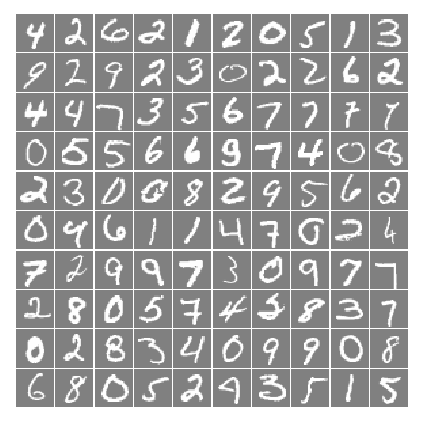
\includegraphics[width=\textwidth]{mnist_sample.png}

The first ten labels in vector \texttt{y} correspond to the digits in the upmost row:  4, 2, 6, 2, 1, 2, 0, 5, 1, 3, as expected.

\color{blue}
\item[(c)] Divide the data into two parts: A 'training set' consisting of the first 2,500 images (and associated labels), and a 'test set' containing the remaining 2,500 images (and their associated labels).

\color{black}
Dividing the data set is simple:
\begin{verbatim}
TrainingSet = X(1:2500,:);
TestSet = X(2501:5000,:);
TrainingSetY = y(1:2500);
TestSetY = y(2501:5000);
\end{verbatim}

\color{blue}
\item[(d)] For each ot the ten classes (digits 0-9), compute a class \textit{prototype} given by the mean of all the images in the training set that belong to this class. That is, select from the training set all images of class '0' and compute the mean image of these; this should look sort of like a zero. Do this for all ten classes, and plot the resulting images. Do they look like what you would expect?

\color{black}
First of all, we need a function to compute the matrix of prototypes (each row of the matrix is a prototype for a specific digit). This ``combined'' approach is solely for efficiency.
\begin{verbatim}
function prototype_matrix = get_prototype_matrix(T, labels)
  prototype_matrix = zeros(10, size(T)(2));
  class_sizes = zeros(1, 10);
  for i = 1:size(T)(1)
    digit = labels(i);
    if digit == 0
      class_sizes(10)++;
      prototype_matrix(10,:) += T(i,:);
    else
      class_sizes(digit)++;
      prototype_matrix(digit,:) += T(i,:);
    endif
  endfor
  for i = 1:10
    prototype_matrix(i,:) /= class_sizes(i);
  endfor
endfunction
\end{verbatim}
Now for each digit $d$, $0 < d < 10$, its prototype is in the matrix' $d$th row, and the prototype for digit 0 is in its 10th row (Matlab/Octave start indexing from 1).

Now, running
\begin{verbatim}
prototype_matrix = get_prototype_matrix(TrainingSet, TrainingSetY);
visual(prototype_matrix);
\end{verbatim}
we will obtain the following output:
\begin{figure}[H]
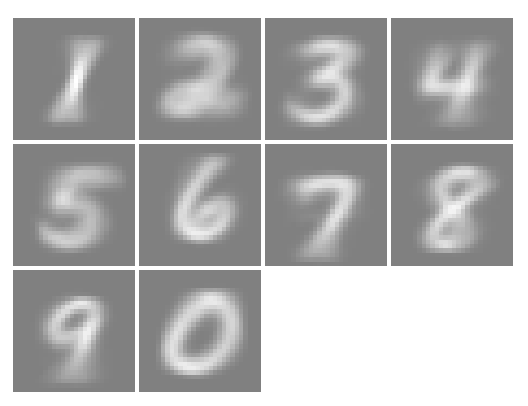
\includegraphics[width=\textwidth, keepaspectratio]{digit_prototypes.png}
\end{figure}
The prototypes look pretty good, but I suspect that 6 and 8 will be confused pretty often.

\color{blue}
\item[(e)] For each of the images in the test set, compute the Euclidian distance of the image to all 10 prototypes, and classify the test image into the class for which the distance to the prototype is the smallest. So, if a test image is closer to the prototype for '3' than it is to the prototypes for any of the other digits, predict its class to be '3'. Compute and display the resulting \textit{confusion matrix}.

\color{black}
Let us implement the naïve classifier:
\begin{verbatim}
function dist = euclidean_distance(a, b)
  dist = norm(a - b);
endfunction

function label = naive_classify_impl(image, prototype_matrix)
  best_digit = -1;
  best_dist = Inf;
  for digit = 1:10
    current_dist = euclidean_distance(image, prototype_matrix(digit,:));
    if best_dist > current_dist
      best_dist = current_dist;
      best_digit = digit;
    endif
  endfor
  if best_digit == 10
    label = 0;
  else
    label = best_digit;
  endif
endfunction

function cm = naive_classify(TestSet, TestSetY, prototype_matrix)
  cm = zeros(10, 10);
  for i = 1:size(TestSet)(1)
    predicted_class = naive_classify_impl(TestSet(i,:), prototype_matrix);
    actual_class = TestSetY(i);
    predicted_class_index = predicted_class;
    actual_class_index = actual_class;
    if predicted_class == 0
      predicted_class_index = 10;
    endif
    if actual_class == 0
      actual_class_index = 10;
    endif
    cm(predicted_class_index, actual_class_index)++;
  endfor
endfunction
\end{verbatim}

Now, to test the classifier with the test data, and to print the resulting confusion matrix, all we need is
\begin{verbatim}
cm1 = naive_classify(TrainingSet, 
                     TrainingSetY, 
                     prototype_matrix)
\end{verbatim}
And the confusion matrix looks as follows:
\begin{verbatim}
   281    20     9     4    16    12    14    13     4     0
     1   192     4     1     1    15     1     9     6     1
     0     4   193     0    14     0     0    25     2     2
     0     5     2   202    11     9    15     4    38     0
     3     2    20     0   136     8     0    20     2     4
     0     2     0     5     2   198     0     1     1     6
     0     2     5     2     6     0   232     1    14     2
     1    11    11     0     1     0     1   150     2     2
     0     1     8    40    11     0    11    15   179     0
     0     2     1     1     9     5     1     2     3   228
\end{verbatim}
where the rightmost column and the bottom row corresponds to digit '0'. The corresponding error rate is 0.2036.

\color{blue}
\item[(f)] Classify each of the test images with a nearest neighbor classifier: For each of the test images, compute its Euclidian distance to all (2,500) of the training images, and let the predicted class be the class of the closest training image. Compute and display the resulting confusion matrix.

\color{black}
The confusion matrix is:
\begin{verbatim}
   283     6     0     3     3     1     3     5     2     0
     0   216     3     0     0     0     2     9     0     0
     0     5   221     0     6     0     0    10     2     2
     1     0     2   231     0     1     6     1    12     0
     1     1    11     0   183     1     0     8     1     1
     0     1     2     0     5   240     0     0     2     1
     1     5     4     2     1     0   257     2    11     0
     0     5     5     0     1     0     0   196     0     0
     0     0     5    19     3     1     7     5   219     0
     0     2     0     0     5     3     0     4     2   241
\end{verbatim}
And the implementation is:
\begin{verbatim}
function predicted_label = knn_classify_impl(TrainingSet,
                                             TrainingSetY,
                                             image)
    best_distance = Inf;
    best_label = -1;
    for i = 1:size(TrainingSet)(1)
      current_dist = euclidean_distance(image, TrainingSet(i,:));
      if best_distance > current_dist
        best_distance = current_dist;
        best_label = TrainingSetY(i);
      endif
    endfor
    predicted_label = best_label;
endfunction

function cm = knn_classify(TrainingSet, TrainingSetY, TestSet, TestSetY)
  cm = zeros(10, 10);
  for i = 1:size(TestSet)(1)
    predicted_digit = knn_classify_impl(TrainingSet,
                                        TrainingSetY,
                                        TestSet(i,:));
    % Map digits 0 to index 10.
    if predicted_digit == 0
      predicted_digit = 10;
    endif
    actual_digit = TestSetY(i);
    if actual_digit == 0
      actual_digit = 10;
    endif
    cm(predicted_digit, actual_digit)++;
  endfor
endfunction

function err_rate = compute_error_rate(cm)
  total = sum(cm(:));
  hits = 0;
  for i = 1:10
    hits += cm(i,i);
  endfor
  err_rate = 1 - hits / total;
endfunction
\end{verbatim}
\color{blue}
\item[(g)] Compute and compare the error rates of both classifiers (the prototype-based classifier and the nearest neighbor classifier). Which is working better? Based on the confusion matrix, which digits are confused with each other? Why do you think this is?

\color{black} The error rate of the prototype-based classifier is 0.2036 and the error rate of kNN-classifier is 0.0852. I think this is due to the fact that kNN works in more global fasion as compared to the prototype-based one, yet the latter provides much better performance.

It seems that digit '8' is getting confused for '3' pretty often, even worse, '3' gets confused to '9' even more frequently. Also '9' gets confused for '4' often.
\end{itemize}

\end{document}